\documentclass[../main/thesis.tex]{subfiles}
\begin{document}
\newchapter
%% my chapter 1 content
\chapter{Testing and Characterization of the 3DMiMic Detector}
\label{3dmimic}

\section{Semiconductors}
\label{t-semi}

A semiconductor is a material with higher resistance than typical resistive materials, like copper, but lower resistance than insulators. Silicon is the most widely used semiconductor element for electronic devices. A semiconductor's conducting properties can be altered by adding different atoms into the crystal lattice. This is called doping. An n-type semiconductor has been doped with atoms containing more free electrons. A p-type similarly has more free holes. Atoms with extra electrons are called donors, and phosphorus is a common donor for silicon doping. Atoms with extra holes are called acceptors, and boron is a common acceptor for silicon doping. \citep[chap. 11]{Knoll}

\subsection{Semiconductor Diodes}

A basic semiconductor diode is based on a pn junction, which is a p-type material in contact with a n-type material. Without an external bias applied, electrons from the n-region near the junction will recombine with holes in the p-region, leaving behind negatively charged ions in the n-region. The opposite happens in the p-region, creating positively charged ions. This creates a region in the junction with a strong electric field, which is called the depletion region, because it is depleted of charge carriers. This makes the depletion region non-conductive. A pn junction is shown in figure \ref{fig-pn}. The depletion region can be made smaller, eventually causing a current to flow, by setting up a voltage across the junction, with the higher potential on the p-side. This is called forward bias. The opposite, reverse bias, causes the depletion region to grow bigger as the charge carriers are pulled away from the junction. \citep[chap. 1]{analogbok}

\begin{figure}%[h]
	\centering
	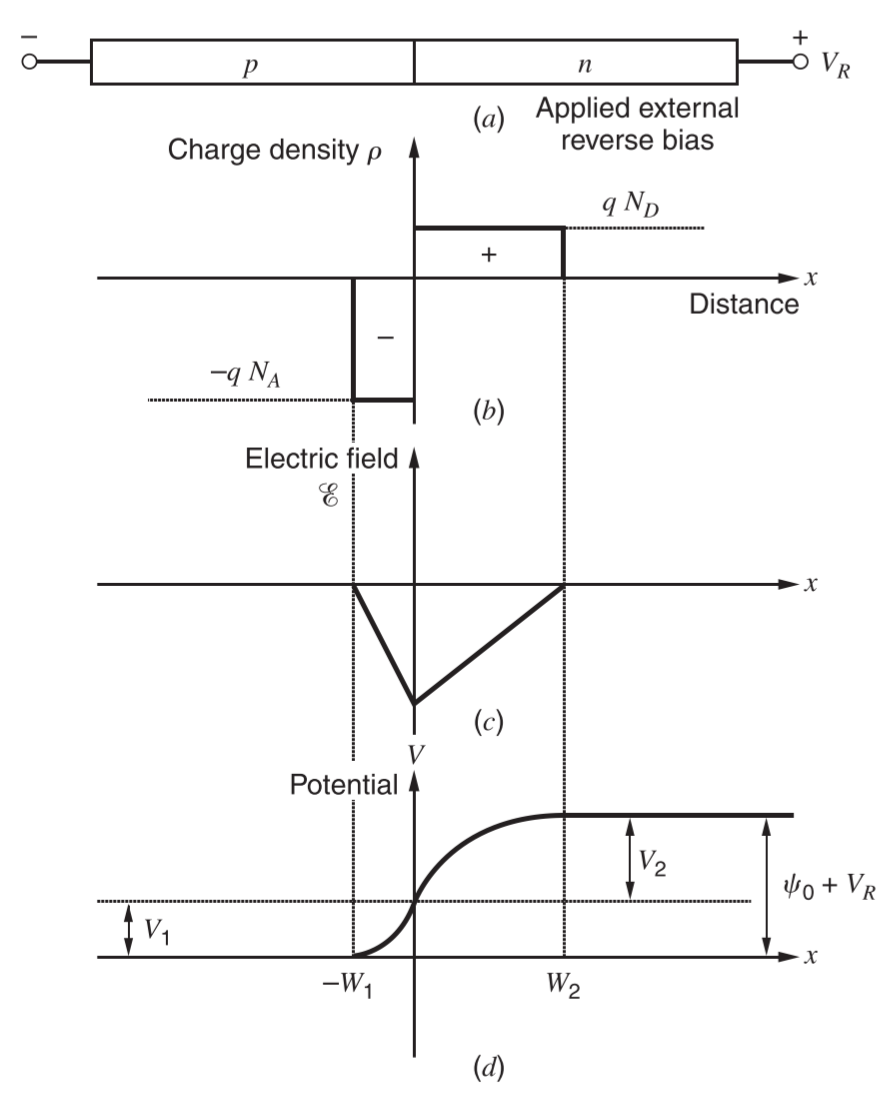
\includegraphics[width=0.5\textwidth]{pn.png}
	\caption{PN junction with depletion region. (a) Schematic. (b) Charge density. (c) Electric field. (d) Electrostatic potential. \citep{analogbok}}
	\label{fig-pn}
\end{figure}

The insulating properties of the depletion region causes only a minimal leakage current to flow during reverse bias. This current is caused by drift, which increases with the electric field up to the point of velocity saturation. The increased interactions between the carriers and the lattice for higher electric fields causes the leakage current to become almost independent of the voltage. This current is often called the reverse saturation current. Once the reverse bias becomes too strong, the high electric field causes the depletion region to break down and high current to flow. This current can break diodes that have not been made to withstand it. Currents for different bias voltages can be seen in figure \ref{fig-pn-iv}. \citep[chap. 1]{analogbok}

\begin{figure}%[h]
	\centering
	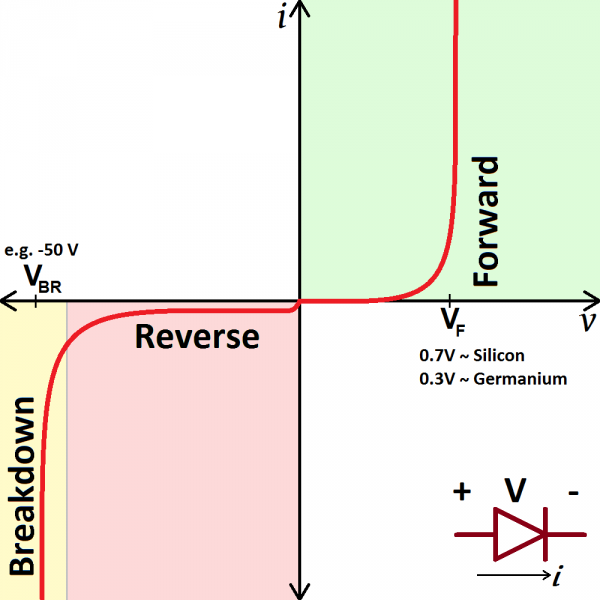
\includegraphics[width=0.4\textwidth]{pn-iv.png}
	\caption{Current-voltage relationship of a diode. \citetext{\citeauthor{SparkFun}}}
	\label{fig-pn-iv}
\end{figure}
%https://learn.sparkfun.com/tutorials/diodes/real-diode-characteristics
%http://www.circuitstoday.com/pn-junction-diode-characteristics

A PIN diode has a large undoped intrinsic semiconductor region between the p-region and n-region. The i-region is flooded with charge carriers from the p- and n-regions. This causes the electric field to cover almost the entire length of the i-region, which speeds up the transport of charge carriers. The depletion region is also independent of the bias voltage. \citep{pin}

\section{Radiation Detectors}
\label{t-detector}
A radiation detector records interactions between incoming radiation and the detector. These interactions could be electrical, chemical, light- or heat-based. Detectors can be based on many different materials, including gas chambers, semiconductors, crystals, and liquid.\comm{\citep[chap. 9]{Thorsteinsen}} In a simple radiation detector a single particle interacts with the detector, resulting in an electric charge appearing inside the detector. This charge is typically collected by setting up an electric field inside the detector, which causes positive and negative charge to flow in opposite directions, forming an electric signal. This signal could be measured as a current (current mode), voltage (mean square voltage mode), or a charge (pulse mode). \citep[chap. 4]{Knoll}

Pulse mode is the most common readout mode because the measurement records each individual quantum of radiation. Pulse mode is therefore required when attempting to measure the energy of individual radiation events. The charge generated in the detector is usually integrated over a certain period of time. Pulse mode, however, does not work well at very high event rates as the time between events becomes too short to analyse the data. Current mode measures the average current over many events, therefore loosing the amplitude and timing information of individual events, but allowing for measurement with high event rates. Mean square voltage mode works much like current mode, but the output signal will be more dependent on the charge per event, making this mode more useful for mixed radiation environments. \citep[chap. 4]{Knoll}

%pulse height spectra, energy resolution, efficiency, dead time


%Dosimeter, microdosimeter?

\subsection{Semiconductor Detectors}
\label{t-detectors-semi}
Semiconductor diode detectors, also called simply semiconductor detectors or solid-state detectors, are radiation detectors employing semiconductor diodes as the basic detection medium. \comm{Silicon is the most common material used, but germanium detectors are superior for gamma-ray measurements. }Semiconductor detectors offer energy resolutions that are superior to other radiation detectors in addition to small size and fast timing characteristics. A big drawback is that they are degraded by radiation-induced damage during normal use. \citep[chap. 11]{Knoll}

Charged particles passing through a semiconductor detector create electron-hole pairs along the particles path. By setting up an electric potential across the diode, there will be an electric field present that will cause the holes to drift in the same direction as the electric field vector, and the electrons in the opposite direction. By monitoring one of the diodes sides, a pulse is measured as the charge from either the holes or the electrons (depending on which side is measured) is collected. 

A semiconductor detector, like other diodes, can be forward biased or reverse biased. It is possible to operate a semiconductor detector without external bias, but it will perform poorly as the electric field across the junction will be too weak to read out the charge carriers before many are lost. Applying forward bias to the detector reduces the electric field even further, while reverse bias increases it. Another important factor is that reverse bias increases the depletion region, which is also the active volume of the detector. \comm{This is the main reason for reverse bias being the dominant choice for radiation detectors.}A PIN diode with its large active volume is therefore very useful as a radiation detector. \citep[chap. 11]{Knoll}

%Tran phd fig 1.3?

%%XXX p-i-n

%%%XXX More details and figures

\section{Semiconductor Characterization}
\label{t-char}

\subsection{Capacitance-Voltage Measurements}
\label{t-cv}
\gls{CV} profiling is a semiconductor characterisation technique that is much used to find doping- and defect densities in semiconductor junctions. The technique relies on the fact that the width of a reverse biased depletion region depends on the applied voltage. The small signal capacitance is dependent on both the doping density and width of the depletion region. \gls{CV} profiles are made by measuring the capacitance while sweeping over a voltage range. The doping density is found from the slope of a C-V curve or a $1/C^2$-V curve. \citep[chap. 2]{Schroder}

There are multiple ways to measure capacitance. A simple method is to supply a known current, and measure how fast the voltage across the capacitor rises. This method assumes an ideal capacitor, and is therefore inaccurate for a real capacitor. A more accurate method is to supply an AC signal to the device under test and measure the AC current and voltage. A high frequency signal ($\sim$10 MHz) will be better for measuring dynamic performance, while a low frequency signal ($\sim$10 kHz) is better to find quasistatic characteristics. The capacitance is calculated from the frequency, current, and voltage. 
%%XXX equation?

%https://en.wikipedia.org/wiki/Capacitance_meter
%http://www.planetanalog.com/document.asp?doc_id=527457
%Paper we got in lab

\subsection{Current-Voltage Measurements}
\label{t-iv}
\gls{IV} characterization is observation of the current through a device when sweeping over the voltage across it. This can be used to find basic electrical parameters for the device. This includes leakage current, resistance, cut-in (threshold) voltage, breakdown voltage, saturation voltage, and hysteresis. 

\section{3DMiMic}
\label{3d-3d}

\begin{figure}%[h]
	\centering
	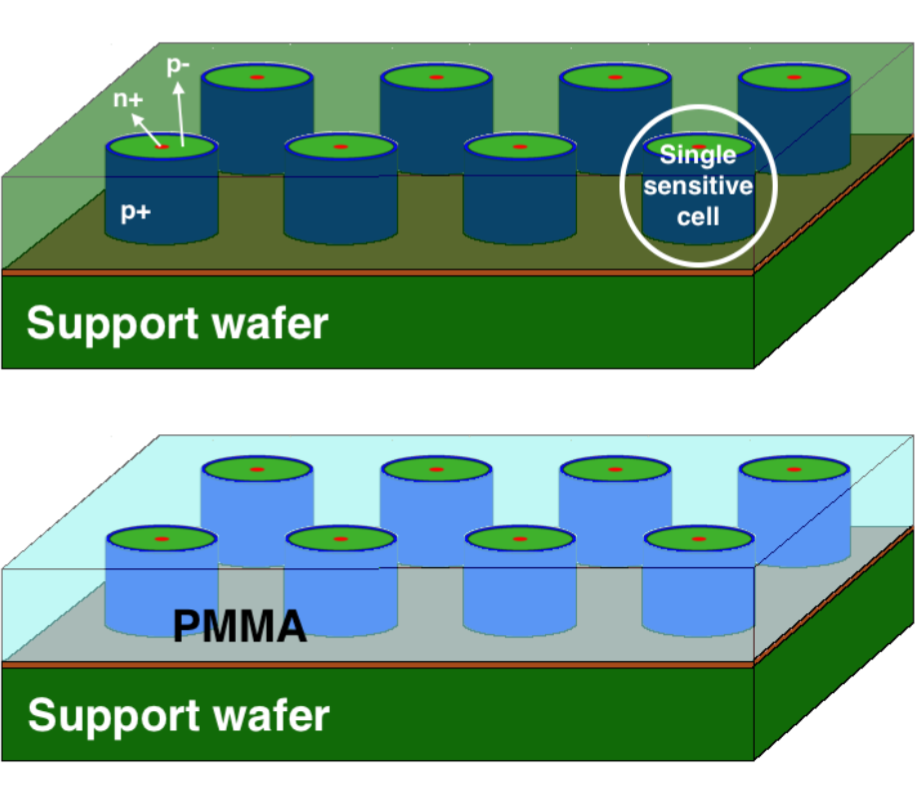
\includegraphics[width=0.6\textwidth]{3dmimic.png}
	\caption{Presentation sketches of the 3DMiMic detector, shown without and with PMMA (tissue equivalent plastic). \citep{Trento2015}}
	\label{fig-3dmimic}
\end{figure}

Si-3DMiMic, or simply 3DMiMic, is a silicon-based 3D mini and micro-dosimeter being developed by SINTEF MiNaLab in Oslo, but was invented and ordered by Professor Anatoly Rozenfeld from the Centre for Medical Radiation Physics at the University of Wollongong. The detector is made to mimic the response of biological tissues to ionizing radiation on a cellular and sub-cellular level, and consists of an array of more than a thousand cylindrical p-i-n diodes (see figure \ref{fig-3dmimic}). This is in an attempt to get a better estimate of the \acrfull{RBE} (section \ref{t-rbe}) by observing the microscopic distribution of the dose. Each diode, or cell, is made of a thin n+ core cylinder, a circular p+ trench some micrometers out, and in some cases a n+ guard ring further away from the core (see figure \ref{fig-3dmimic-top-side}). There are multiple versions of the detectors, with differences including presence of n+ guard ring, size of cell, and structure. The silicon between the different cells should be etched away and replaced with tissue equivalent \gls{PMMA}, but this has not been attempted by SINTEF yet as of the time this thesis is written. This should be done because \gls{PMMA} produces secondary radiation in a very similar way to how tissue does, unlike silicon, due to the mass numbers of the atoms. 
%some are 50x50

%Each diode, or cell, is made of a 3 $\mu$m diameter n+ core cylinder, a 2 $\mu$m thick p+ trench about 10 $\mu$m further out, and a 4 $\mu$m thick n+ ring about 20 $\mu$m outside the core. The silicon between the different cells has been etched away and replaced with tissue equivalent \gls{PMMA}. %Need to double check all this later, I have contradicting sources

Figure \ref{fig-3dmimic-side} show a "3D" layout with the n+ core cylinder and the p+ trench going all the way through the bulk, and a planar n+ guard ring. There also exist designs with either or both the n+ core and p+ trench made planar. There are designs with cells in two different sizes, seen in figure \ref{fig-top-both}. The radii of the p+ trench circles are roughly 15 and 20 $\mu$m for the two designs. The detectors with the smaller diodes have 50x50 cells, while the larger variant has 32x33 or 33x33 cells depending on the layout. Images of some of the different layouts can be found in Appendix \ref{a-3dmimic-layout}.
%Figure \ref{fig-3dmimic-top15} shows the smallest, "15 $\mu$m", layout of 3DMiMic from above with a size scale.


%\begin{figure}%[h]
%	\centering
%	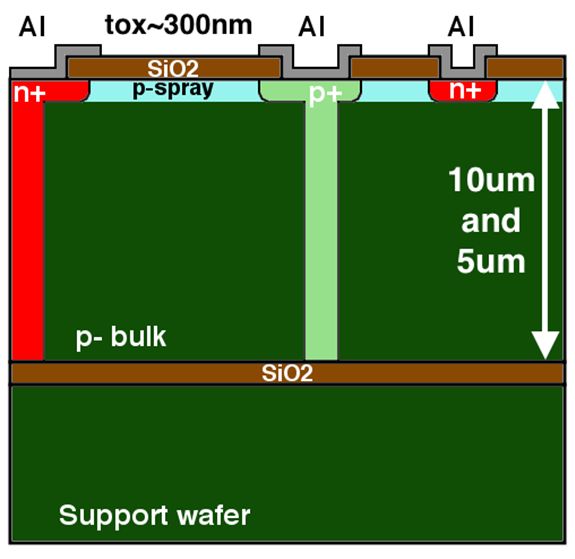
\includegraphics[width=0.5\textwidth]{3d-side.png}
%	\caption{Layout of 3DMiMic design with 3D n+ core and 3D p+ trench. \citep{Marco}}
%	\label{fig-3dmimic-side} %need to check permission
%\end{figure}

\begin{figure}
	\centering
	\begin{subfigure}{.5\textwidth}
		\centering
		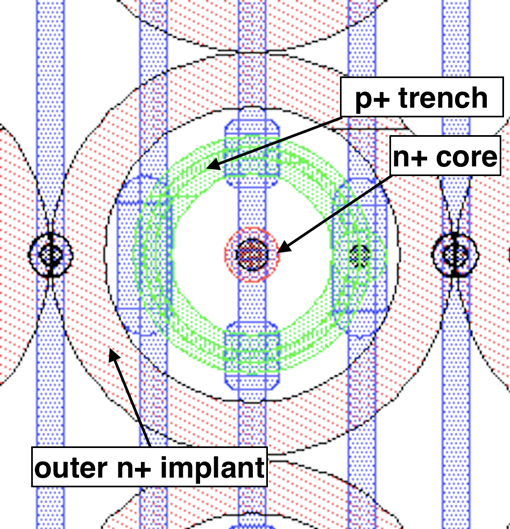
\includegraphics[width=.9\linewidth]{3d-top.png}
		\caption{Top view with guard ring present.}
		\label{fig-3dmimic-top}
	\end{subfigure}%
	\begin{subfigure}{.5\textwidth}
		\centering
		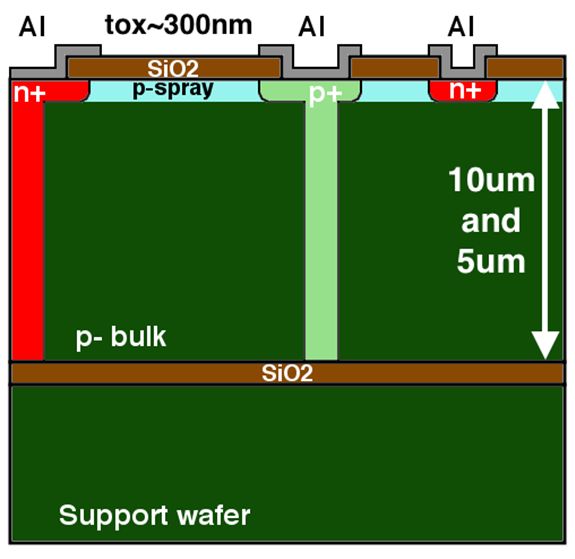
\includegraphics[width=\textwidth]{3d-side.png}
		\caption{Side view with 3D n+ core, 3D p+ trench, and planar n+ guard.}
		\label{fig-3dmimic-side} %need to check permission
	\end{subfigure}
	\caption{Layout of a 3DMiMic cell. \citep{Marco}}
	\label{fig-3dmimic-top-side}
\end{figure}


%\begin{figure}[h]
%	\centering
%	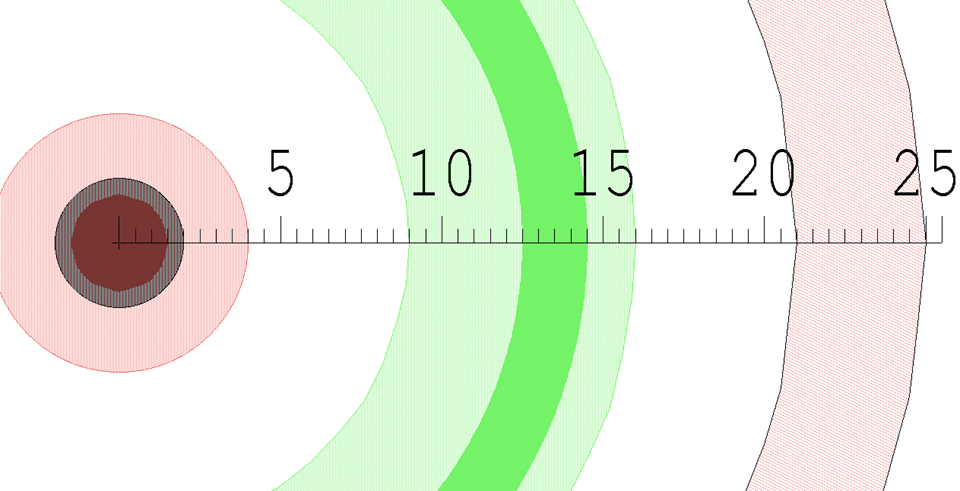
\includegraphics[width=0.7\textwidth]{3d-top15.png}
%	\caption{Smallest, "15 $\mu$m", layout of 3DMiMic seen from above. Shows a zoom of figure \ref{fig-3dmimic-top} with a distance scale is in $\mu$m. \citep{Marco}}
%	\label{fig-3dmimic-top15} %need to check permission
%\end{figure}

In the main layout of 3DMiMic, all the n+ cores in a line is connected together. Every second line is also connected, leaving two channels (odd/even) for readout. When present, all the outer n+ rings are connected and can be read out if desired. A full die is shown in figure \ref{fig-3dmimic-die}, where the "+" pads are the n+ cores, the "G" pads are for the p+ trenches, the "GUARD" pads are for the cell guard rings, and the large square around the detector is a guard ring. There also exist other layouts, for example with all diodes connected together, readout in eight channels, and a larger design made to be bump bonded to a Medipix chip (see section \ref{e-medipix}). 

\begin{figure}%[h]
	\centering
	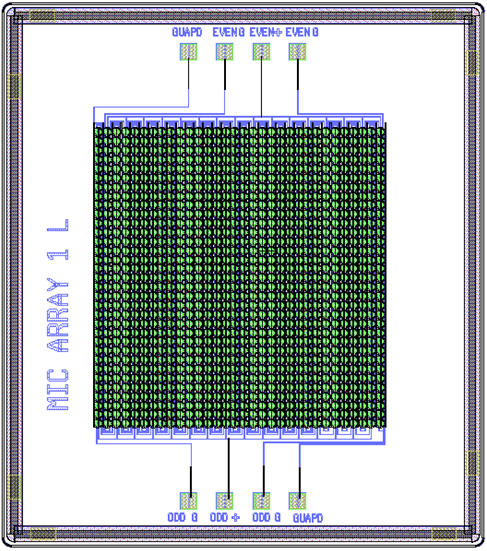
\includegraphics[width=0.7\textwidth]{3d-die.png}
	\caption{Layout of a full 3DMiMic die, showing bonding pads and the guard ring outside the active area. \citep{Marco}}
	\label{fig-3dmimic-die} %need to check permission
\end{figure}

Even though the odd/even readout scheme contains two channels, it does not provide any spacial information, as both channels cover the whole active area of the detector. The reason for this layout is to notice if a particle track goes through multiple adjacent cells. If both readout channels are triggered at the same time, this was not a single event, as it will look if all cells are read in a single channel.

\subsection{3DMiMic Response to Radiation}
Table \ref{tab-3d-response} show the expected signal strength from the 3DMiMic detectors to a \gls{MIP}, a proton in the Bragg peak, and a carbon ion in the Bragg peak. The proton and carbon numbers are from Geant4 simulations done by Andreas Samnøy. The \gls{MIP} numbers are calculated from the minimum stopping power for a proton in silicon. The table also show safety margins that are a bit higher than the expected signal. The electronics should be able to read out signals of at least the safety margins in case of simulation inaccuracies. The radiation will also deposit slightly more energy of they pass through the detector volume diagonally. 

\begin{table}[h!]
	\begin{center}
		\caption{Simulated response from some types of radiation. \citep{Samnoy}}
		\label{tab-3d-response}
		\begin{tabular}{lccc}\toprule
			\textbf{Radiation}           &           &\textbf{Deposited energy} &          \\
			& {[}keV{]} & {[}fC{]}         & {[}e-{]} \\ \midrule
			MIP                  & 3.87      & 0.172         & 1075     \\
			Proton in Bragg      & 680       & 30            & 189k     \\
			\textit{(with safety margin)} & 1080      & 48            & 300k     \\
			Carbon in Bragg      & 12000     & 533           & 3.3M     \\
			\textit{(with safety margin)} & 14400     & 640           & 4M	\\
			\bottomrule
		\end{tabular}
	\end{center}
\end{table}

Table \ref{tab-3d-response} sets the requirements for the readout electronics' dynamic range to between 1000 and 4 million electrons, which is equivalent to a range of 4000:1. A range this long can be very difficult to get without sacrificing too much of the other properties of the electronics. One possible method of reducing the required dynamic range is to exploit the odd / even readout scheme. The dynamic range can be split in two, one range for each readout channel. Then half the pixels can be used to read the smallest particles, and the other half can read the largest particles. 

\section{I-V Measurements of 3DMiMic Detectors on Wafer}
\label{3d-IV}

\begin{figure}%[h]
	\centering
	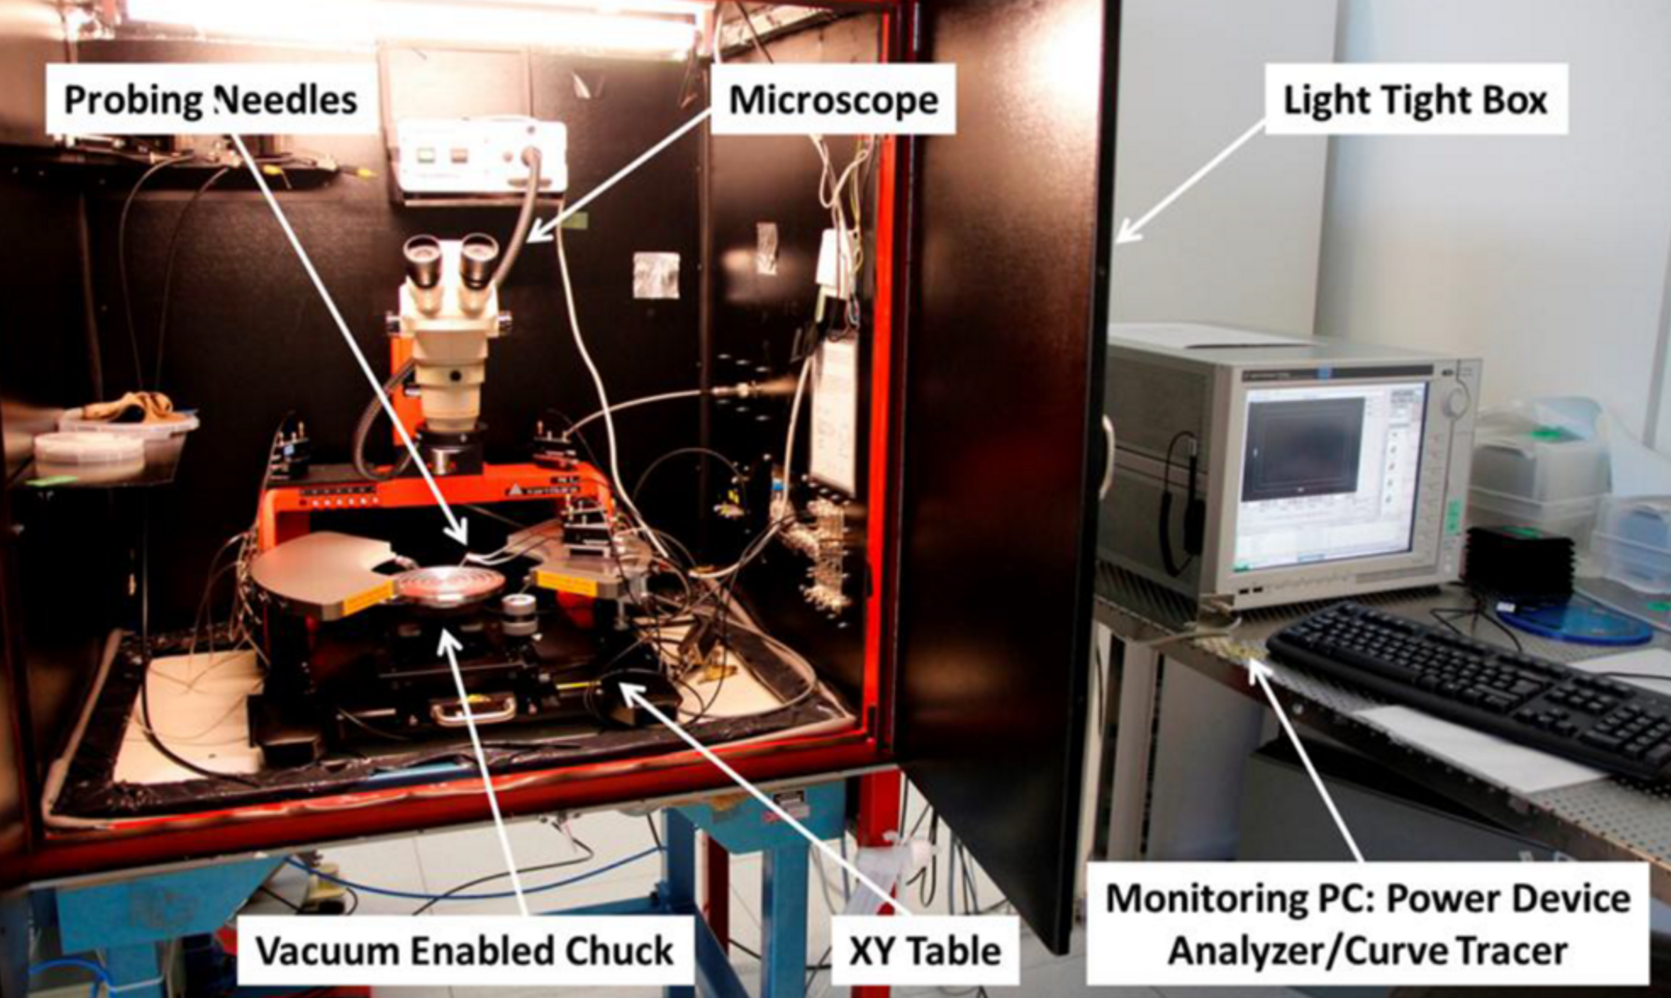
\includegraphics[width=0.8\textwidth]{SINTEF_probe.png}
	\caption{Equipment setup for I-V measurements at SINTEF. \citep{Yashika}}
	\label{fig-3d-probe} 
\end{figure}

\gls{IV} measurements of seven 3DMiMic wafers where performed in the cleanroom at SINTEF MiNaLab in Oslo by Øyvind Lye and Andreas Tefre Samnøy in May 2016. The equipment setup is shown in figure \ref{fig-3d-probe}. These seven wafers have been produced with different designs and fabrication processes, see appendix \ref{a-3dmimic-layout}. Each wafer has 104 detectors with odd/even readout, 6 detectors with single channel readout, and several other experimental layouts. The detectors had to be tested with manual needle placement, as the designs are too different to use an automatic system with a probe card. The wafer is held in place on a stand using vacuum, and the stand can be moved in the horizontal plane. The needles can be manually placed at the desired location, and the position can be fine-tuned in Cartesian space using screws. The cell n+ guard ring was not connected on the detectors where it is present. This was done because it would require a separate test setup for the detectors with the ring, which would increase the time needed for the measurement. A total of 580 detectors were measured. 

\begin{figure}%[h]
	\centering
	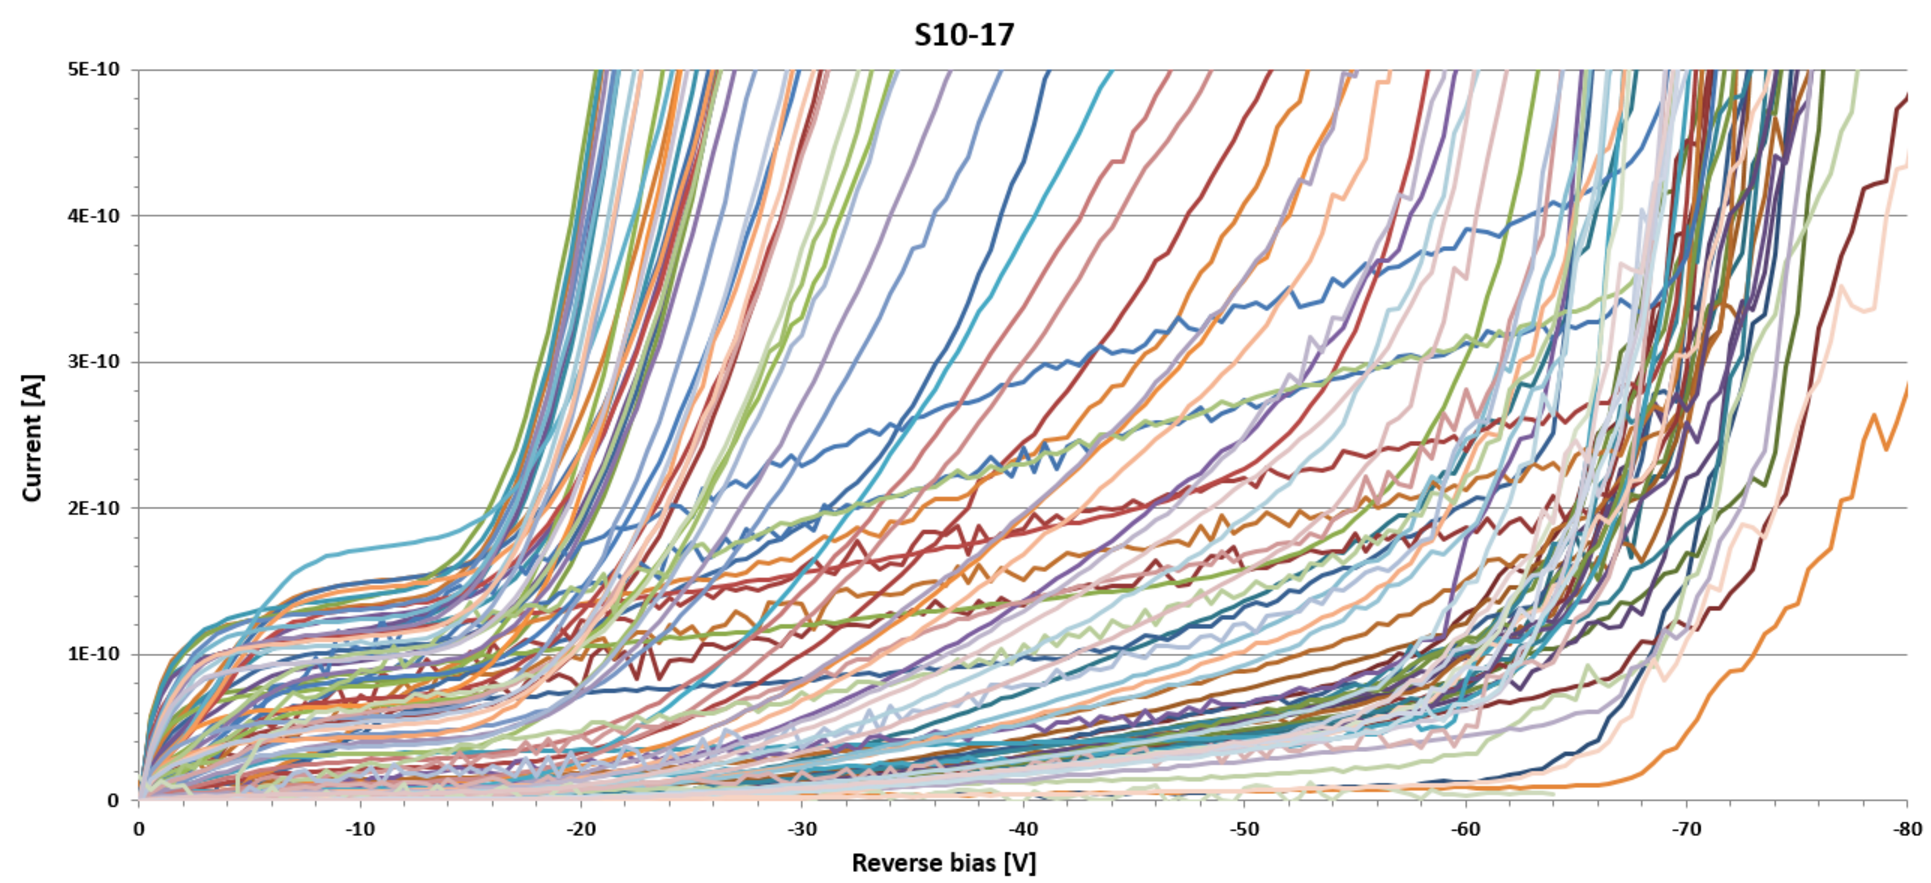
\includegraphics[width=\textwidth]{S10-17.png}
	\caption{I-V measurement of the S10-17 wafer. }
	\label{fig-3d-S10-17} 
\end{figure}

\begin{figure}%[h]
	\centering
	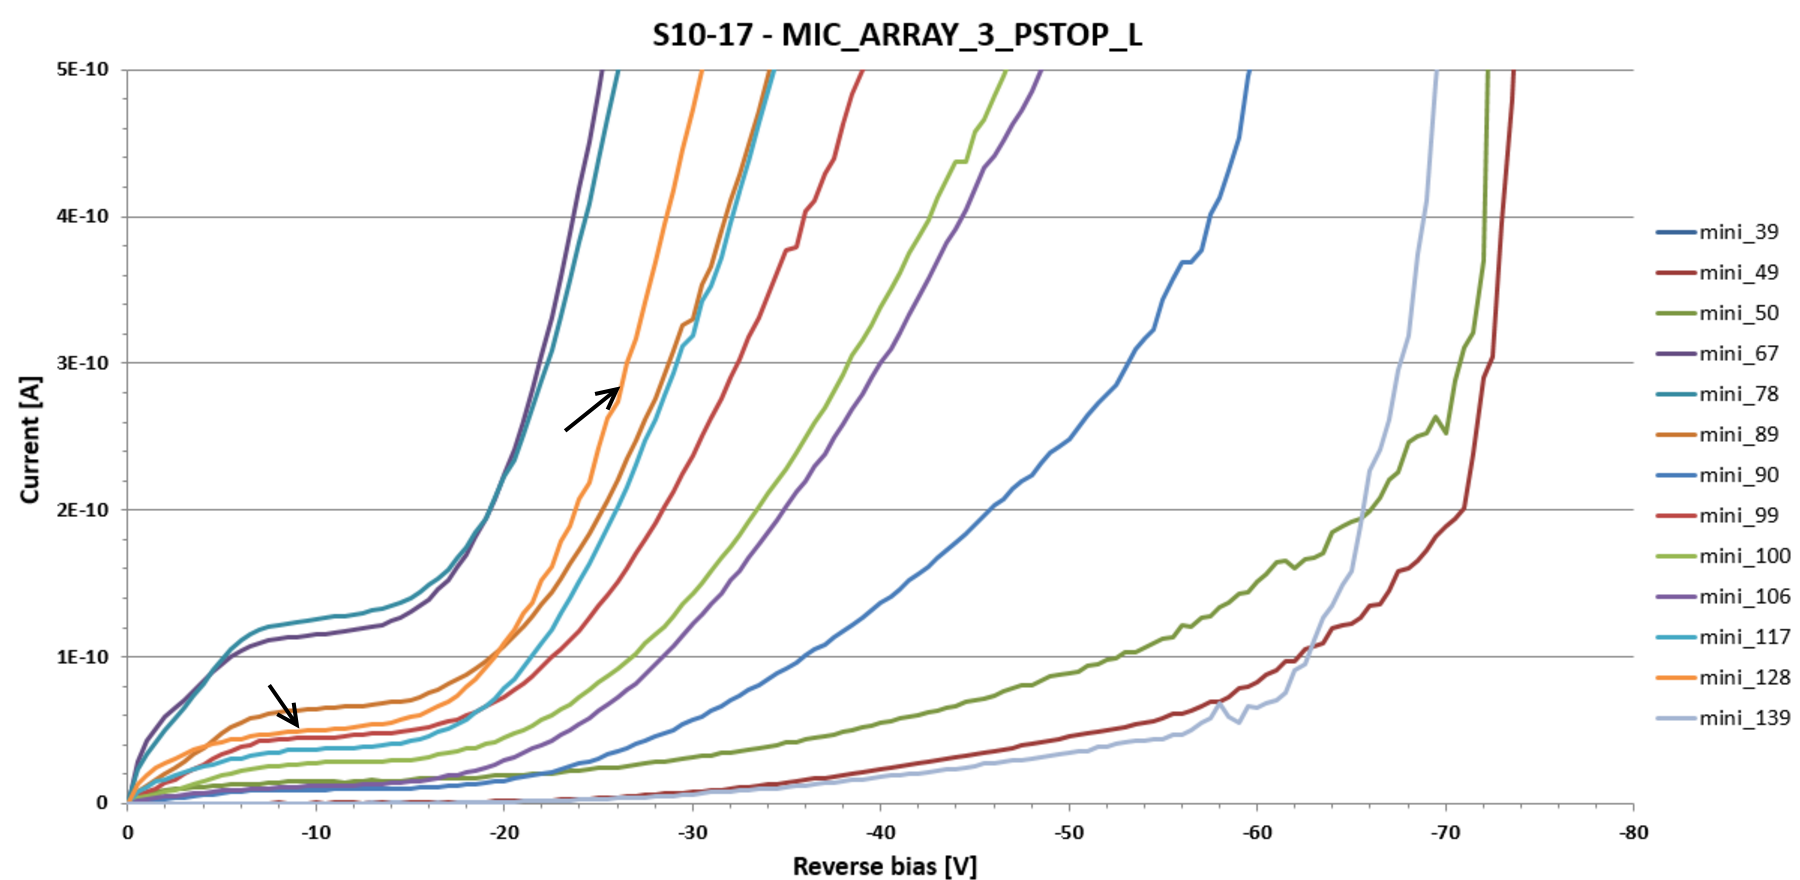
\includegraphics[width=\textwidth]{S10-17-PSTOP_L.png}
	\caption{I-V measurement of the S10-17 MIC\_ARRAY\_3\_PSTOP\_L detectors. S10-17 \#128 marked with arrows.}
	\label{fig-3d-S10-17-PSTOP_L} 
\end{figure}

All measurements can be seen in appendix \ref{a-iv}. As an example, figure \ref{fig-3d-S10-17} shows the measurements from all the measured detectors on wafer S10-17. This clearly shows the huge differences between the detectors. This is also partly because there are multiple different layouts on one wafer, but figure \ref{fig-3d-S10-17-PSTOP_L} also shows large differences between the detectors of one layout. This is not very surprising, as the 3DMiMic detectors are made of very small, complex structures. Small variations in the production process, for example etching acting at different speeds on different parts of the wafer, can make a huge impact, especially if contacts to multiple pixels are broken. It would be interesting to test the number of dead pixels on the detector. This has previously been done at \gls{uib} by scanning a detector with a laser while moving the detector with an XY table. The laser point must be precise enough to not hit two pixels at once, and the XY table must be able to perform steps smaller than the distance between two pixels.  

In general, wafers S10-1, S10-2, S10-11, S10-16 break down very early. S10-16 has a few good looking plateus, but most of them are at very high currents. S10-15 currents increase rapidly and do not saturate. S10-14 also lacks the plateau curves. S10-4 has many relatively nice curves, but also many that rise too rapidly. S10-17 has the most curves with a nice saturation plateau at a not too high current. Which of the layouts that show the best characteristics varies a bit between the wafers, but MIC\_ARRAY\_3, 3\_L, PSTOP, and 3\_PSTOP\_L seem to show the best characteristics. In general, MIC\_ARRAY\_1 and 2 seem to show the worst characteristics. 

\section{Detector Interface PCB}
\label{3d-pcb}
A \gls{PCB}, see figure \ref{fig-3dmimic-photo}, was designed to interface 3DMiMic to the supply and readout electronics. This could have been very simple, but after discussions with Marco at SINTEF it was decided to make it as multi-purpose as possible with possibilities for quick reconnection for different setups. One of the main reasons for this was that the PCB was designed months before the detectors were finished. The PCB is described in detail in appendix \ref{a-pcb}.

\begin{figure}[h]
	\centering
	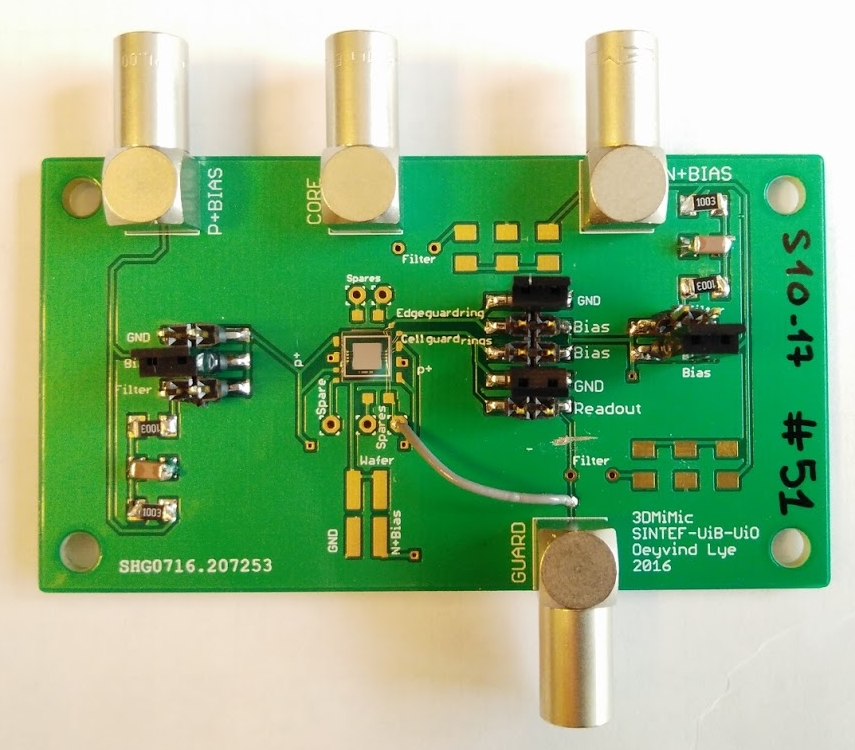
\includegraphics[width=0.7\textwidth]{3dmimic.jpg}
	\caption{Photo of 3DMiMic detector on PCB.}
	\label{fig-3dmimic-photo}
\end{figure} 

\newpage
\section{Wire Bonding}
Wire bonding the detectors to the PCB was supposed to be performed by SINTEF, but they had problems with the wire bonder in June 2016 which would have led to another delay. To avoid this delay, three detectors glued to PCBs were picket up at SINTEF and brought to the cleanroom at Vestfold Innovation Park for wire bonding. The wire bonder was already loaded with 17.5 $\mu$m gold wire, and this was used even though it is thinner than necessary for the 3DMiMic detectors. Each connection was done with two parallel wires for redundancy in case of mechanical damage to the thin wires. The three detectors are numbered: S10-15 $\#$128 (MIC$\_$ARRAY$\_$3$\_$PSTOP$\_$L layout), S10-17 $\#$51 (MIC$\_$ARRAY$\_$1 layout), and S10-17 $\#$128 (MIC$\_$ARRAY$\_$3$\_$PSTOP$\_$L layout). See appendix \ref{a-3dmimic-layout} for the differences in the wafers and layouts, and appendix \ref{a-pcb} for bonding schematics. 

\section{I-V Measurements of 3DMiMic Detectors on PCB}
\label{3dmimic-iv-pcb}

The I-V measurements in Bergen has been done with the Keithley 2635A sourcemeter, controlled by a LabVIEW program made by Enver Alagoz. The positive bias is set to the odd or even readout pin, while the p+ ring is connected to ground through the ground plane and the shielding of the bias wire. The exception to this is one measurement where ground is connected to the p+ ring with the separate p+ LEMO connector. 

Both sides (odd/even) of the three detectors brought to Bergen have been repeatedly measured over a period of 1.5 months. The odd sides of both S10-17 \#128 and S10-17 \#51 appear to be short-circuited. Since the only measurements from SINTEF are the even sides of S10-17 \#128 and S10-17 \#51, it is unclear if the problem is on the detector, or on the \gls{PCB}. For the S10-17 \#51 it is considered likely that the wire bonding is the cause, as this is bonded according to figure \ref{fig-wire-2-g}. The bond on the odd side is very long and difficult to perform. Microscope observations show that the bond is very close to, and possibly touching the edge of the detector. The S10-17 \#51, which has guard rings for every pixel, was tested with guard rings disconnected and connected to ground. This showed no difference on the I-V measurements, so the rest of the measurements have been done with the guard rings connected to ground. 

\begin{figure}[p]
	\centering
	\begin{subfigure}{.5\textwidth}
		\centering
		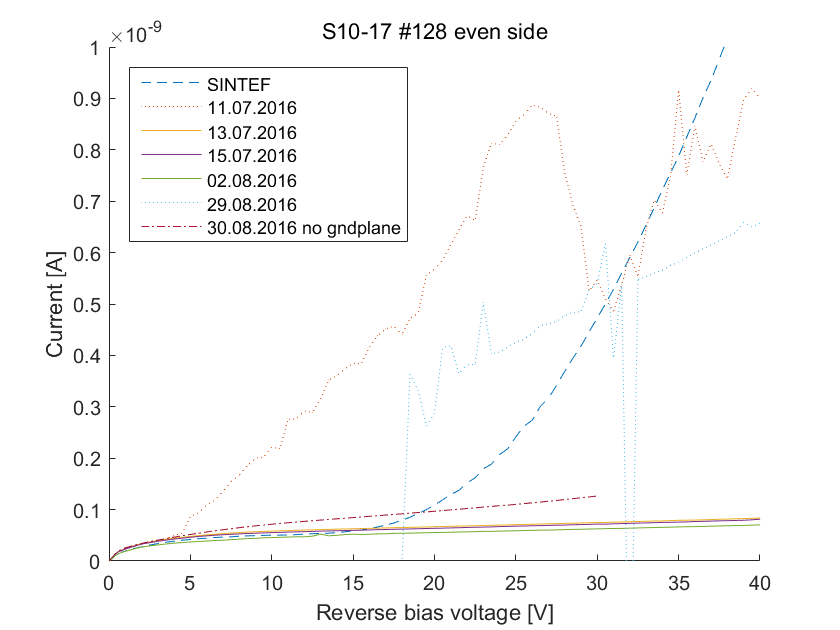
\includegraphics[width=\textwidth]{S10-17-128-e.png}
		\caption{S10-17 \#128 even side.}
		\label{fig-S10-17-128-e}
	\end{subfigure}%
	\begin{subfigure}{.5\textwidth}
		\centering
		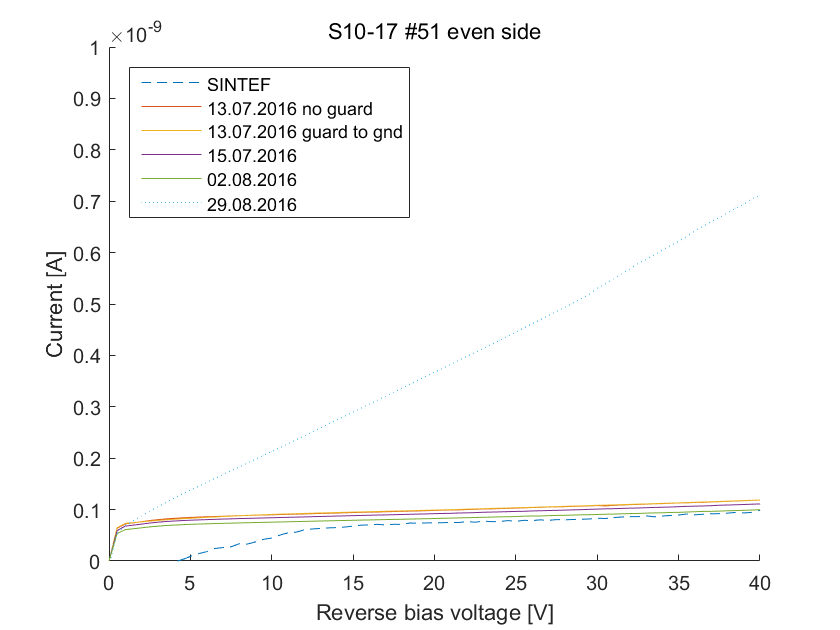
\includegraphics[width=\textwidth]{S10-17-51-e.png}
		\caption{S10-17 \#51 even side.}
		\label{fig-S10-17-51-e} 
	\end{subfigure}
	\caption{I-V measurements of S10-17 detectors on PCB.}
	\label{fig-3d-iv-S10-17}
\end{figure}

\begin{figure}[p]
	\centering
	\begin{subfigure}{.5\textwidth}
		\centering
		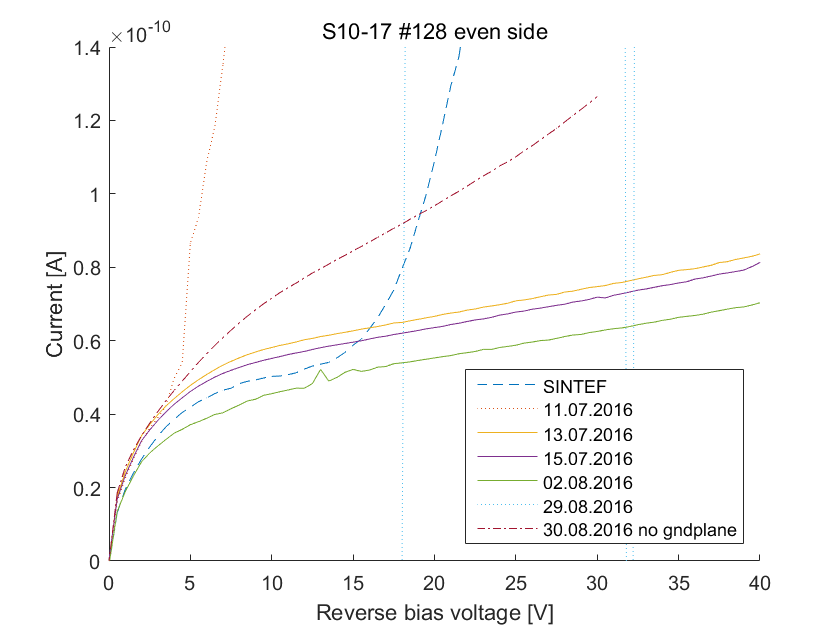
\includegraphics[width=\textwidth]{S10-17-128-e-z.png}
		\caption{S10-17 \#128 even side.}
		\label{fig-S10-17-128-e-z}
	\end{subfigure}%
	\begin{subfigure}{.5\textwidth}
		\centering
		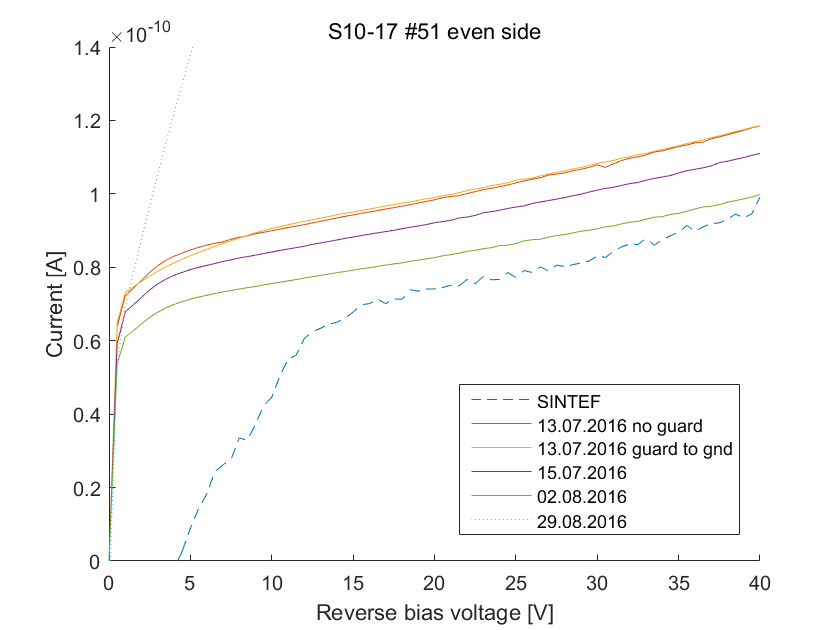
\includegraphics[width=\textwidth]{S10-17-51-e-z.png}
		\caption{S10-17 \#51 even side.}
		\label{fig-S10-17-51-e-z} 
	\end{subfigure}
	\caption{I-V measurements of S10-17 detectors on PCB. Zoom on flat area.}
	\label{fig-3d-iv-S10-17-z}
\end{figure}

\begin{figure}[p]
	\centering
	\begin{subfigure}{.5\textwidth}
		\centering
		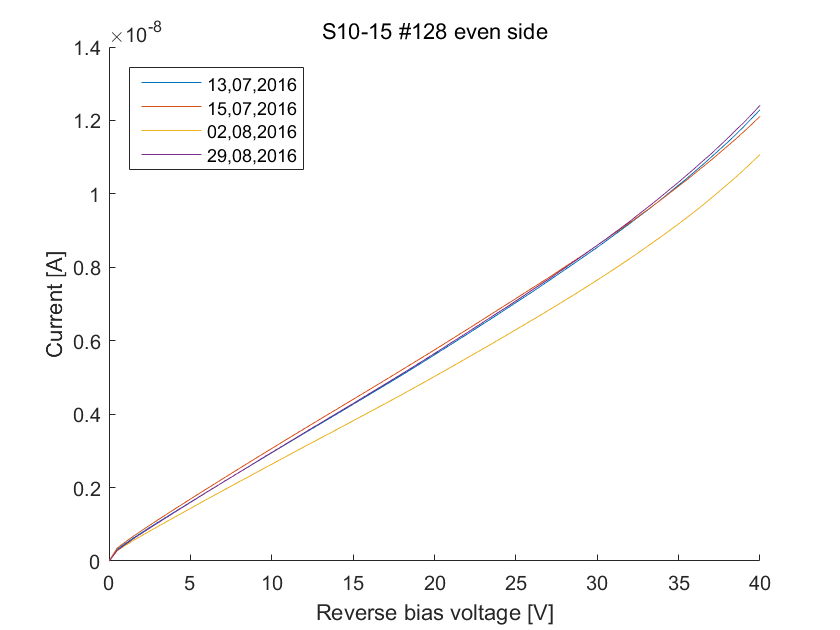
\includegraphics[width=\textwidth]{S10-15-128-e.png}
		\caption{S10-15 \#128 even side.}
		\label{fig-S10-15-128-e}
	\end{subfigure}%
	\begin{subfigure}{.5\textwidth}
		\centering
		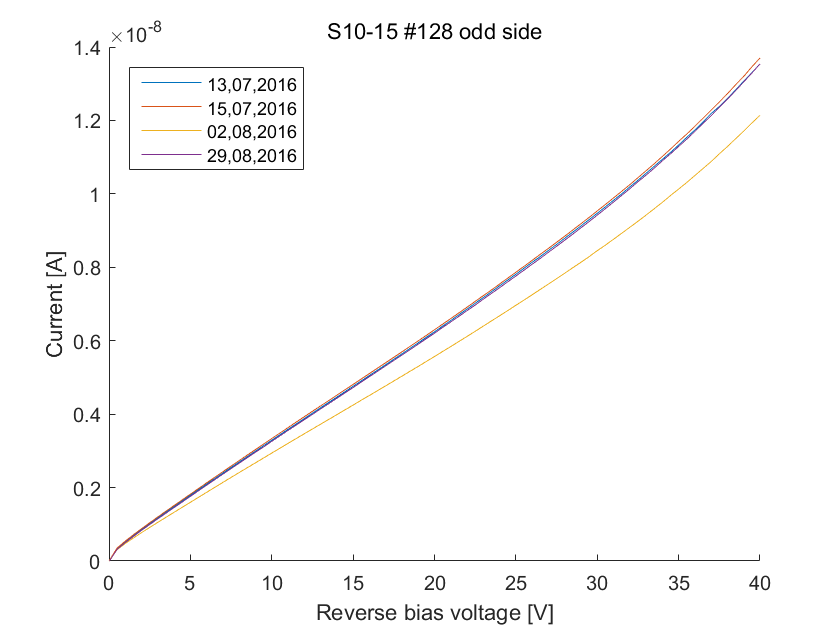
\includegraphics[width=\textwidth]{S10-15-128-o.png}
		\caption{S10-15 \#128 odd side.}
		\label{fig-S10-15-128-o}
	\end{subfigure}
	\caption{I-V measurements of S10-15 detectors on PCB.}
	\label{fig-3d-iv-S10-15}
\end{figure}

Figures \ref{fig-3d-iv-S10-17} and \ref{fig-3d-iv-S10-15} show the I-V measurements performed at \gls{uib} together with the corresponding measurements from SINTEF (dashed line). The S10-17 detectors show a large range where the current has saturated at a fairly low leakage current, see figure \ref{fig-3d-iv-S10-17-z}. The measurements do not fit perfectly with the SINTEF measurements however, because the S10-17 \#128 went into breakdown much earlier at SINTEF, and the S10-17 \#51 saturated much later. The reason behind this is unclear, as this should not be affected by the \gls{PCB}. The slow saturation of the S10-17 \#51 could be due to bad needle contact during the SINTEF measurement. There is also two \gls{uib} measurements for S10-17 \#128, and one for S10-17 \#51 (dotted line) that do not fit with the others. These have very strange behaviour, and is likely caused by equipment malfunction, for example bad cables can have a significant effect on currents as low as this. The S10-15 measurements are very consistent, but the current does not saturate, and is much higher than on the S10-17 detectors. The measurement performed with ground on a separate LEMO cable (dash-dotted line) does not fit with the SINTEF measurement, which is strange. All of the measurements show breakdown between 60 and 80~V (not shown in the figures). 

%show a drop in current over time. If this continues, it could be an issue. It should also be investigated if this drop is caused by the measuring equipment, and not the detectors. 

\newpage
\section{C-V Measurements of 3DMiMic Detectors}

C-V measurements have been performed in Bergen with the HP 4263B LCR meter and Keithley 2635A sourcemeter, controlled by a LabVIEW program made by Enver Alagoz. Ground is connected to p+ through a separate cable to the p+ connector. 

\begin{figure}[h!]
	\centering
	\begin{subfigure}{.5\textwidth}
		\centering
		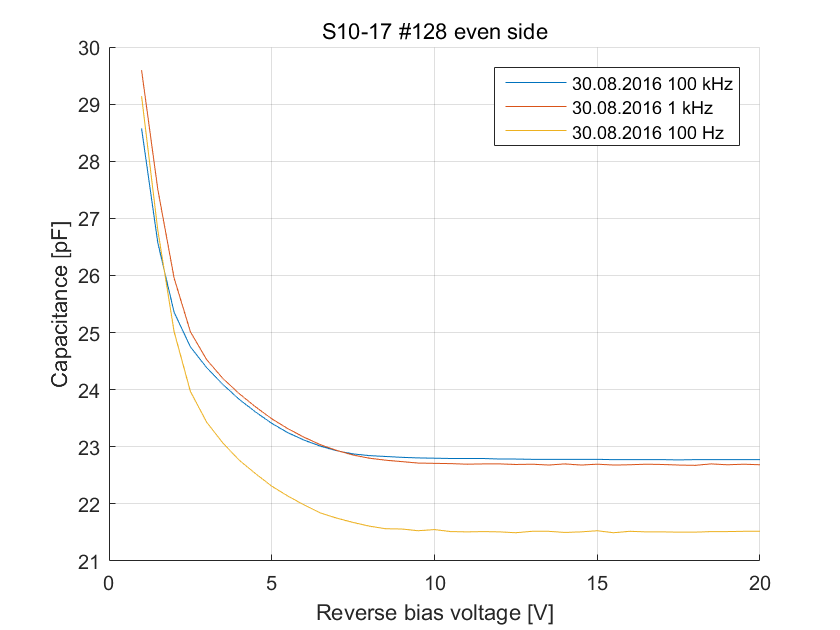
\includegraphics[width=\textwidth]{cv-S10-17-128-e.png}
		\caption{S10-17 \#128 even side.}
		\label{fig-cv-S10-17-128-e}
	\end{subfigure}%
	\begin{subfigure}{.5\textwidth}
		\centering
		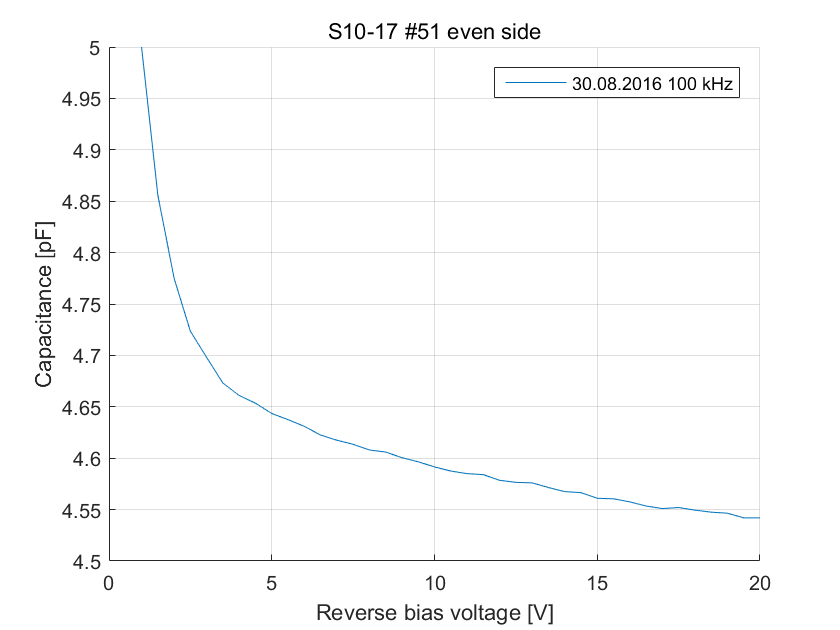
\includegraphics[width=\textwidth]{cv-S10-17-51-e.png}
		\caption{S10-17 \#51 even side.}
		\label{fig-cv-S10-17-51-e} 
	\end{subfigure}
	\caption{C-V measurements of S10-17 detectors on PCB.}
	\label{fig-3d-cv-S10-17}
\end{figure}

\begin{figure}[h!]
	\centering
	\begin{subfigure}{.5\textwidth}
		\centering
		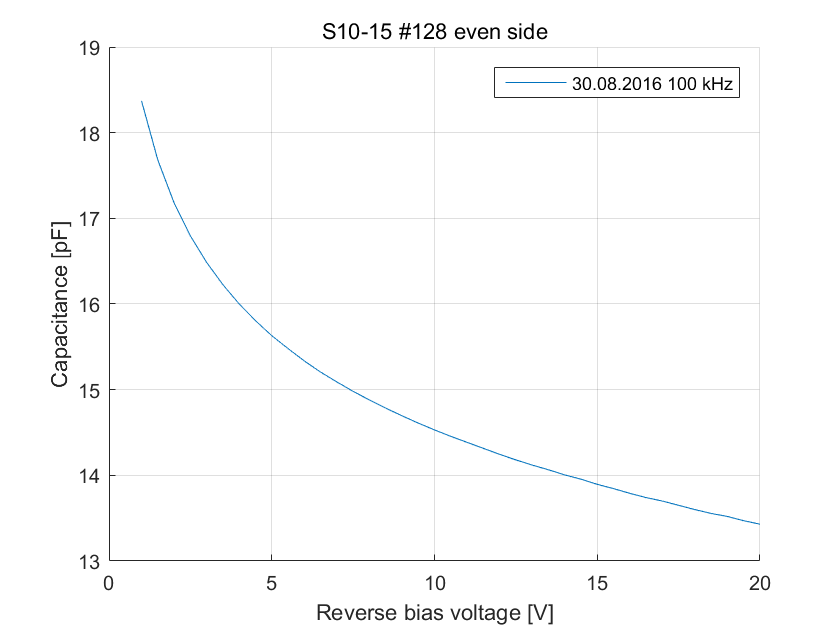
\includegraphics[width=\textwidth]{cv-S10-15-128-e.png}
		\caption{S10-15 \#128 even side.}
		\label{fig-cv-S10-15-128-e}
	\end{subfigure}%
	\begin{subfigure}{.5\textwidth}
		\centering
		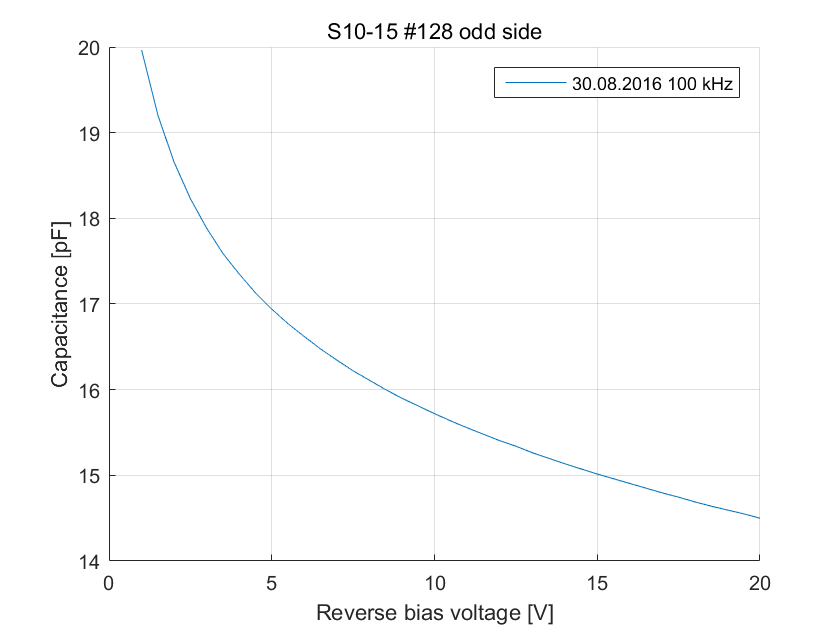
\includegraphics[width=\textwidth]{cv-S10-15-128-o.png}
		\caption{S10-15 \#128 odd side.}
		\label{fig-cv-S10-15-128-o}
	\end{subfigure}
	\caption{C-V measurements of S10-15 detectors on PCB.}
	\label{fig-3d-cv-S10-15}
\end{figure}

The expected capacitance value from simulations from \gls{UOW} was about 20 to 30~pF for the detectors with large pixels. These measurements therefore show very good results, with the highest value of less than 23~pF at 10~V. Assuming every pixel is connected and no capacitance from wires etc., the capacitance per pixel is 21~fF, 2~fF, 14~fF, and 15~fF at 10~V for the four detectors in the order they are shown in the figures. 

\newpage
\section{Radiation Measurements with Americium source}

A few radiation measurements have been performed in Bergen with an Americium-241 source after the detectors were received. Am-241 has a half-life of 432.2 years, and decays by releasing an alpha (helium-4 nucleus) and a photon. The alpha energy is 5.486~MeV 85~\% of the time, 5.443~MeV 13~\% of the time, and 5.388~MeV 2~\% of the time. The most common photon  energy is 59.54~keV. \citep{Lund} The even sides of the detectors from section \ref{3dmimic-iv-pcb} have been tested and seem to be working. Figures \ref{fig-3dmimic-am-17-128-10} and \ref{fig-3dmimic-am-17-128-25} show measurements with the S10-17~\#128 detectors. These were measured with 10~V bias voltage on the detectors, and the Americium source at two different distances from the detector in order to attenuate the beam before reaching the detector, giving two different spectrums. The detectors were read out with the Ortec 142A pre-amplifier and the Caen V1729A ADC. The 10 and 25~mm measurements were taken over roughly 38 and 72~hours respectively. The figures show that the histogram consists of two Gaussians. The second, lower (in counts) Gaussian is for the radiation particles that pass through the metal on top of the pixel before entering the detector volume. This is much lower in number of counts, because the metal covers only a small part of the active volume. 

The deposited energy is higher for longer distance between the source and detector, because the increased distance causes the Bragg peak to be closer to the detector. In figure \ref{fig-3dmimic-am-17-128-10} the peak from the alpha particles passing through the metal is at higher energy because the metal slows the particles, causing the Bragg peak to move closer. After going through 2.5~cm of air, the alphas will have lost a lot of energy, which makes them loose a lot of energy when passing he aluminium layer. They therefore have little energy left to deposit in the sensitive volume. This is why the lower Gaussian is to the left of the main Gaussian in figure \ref{fig-3dmimic-am-17-128-25}. 

\begin{figure}[p]
	\centering
	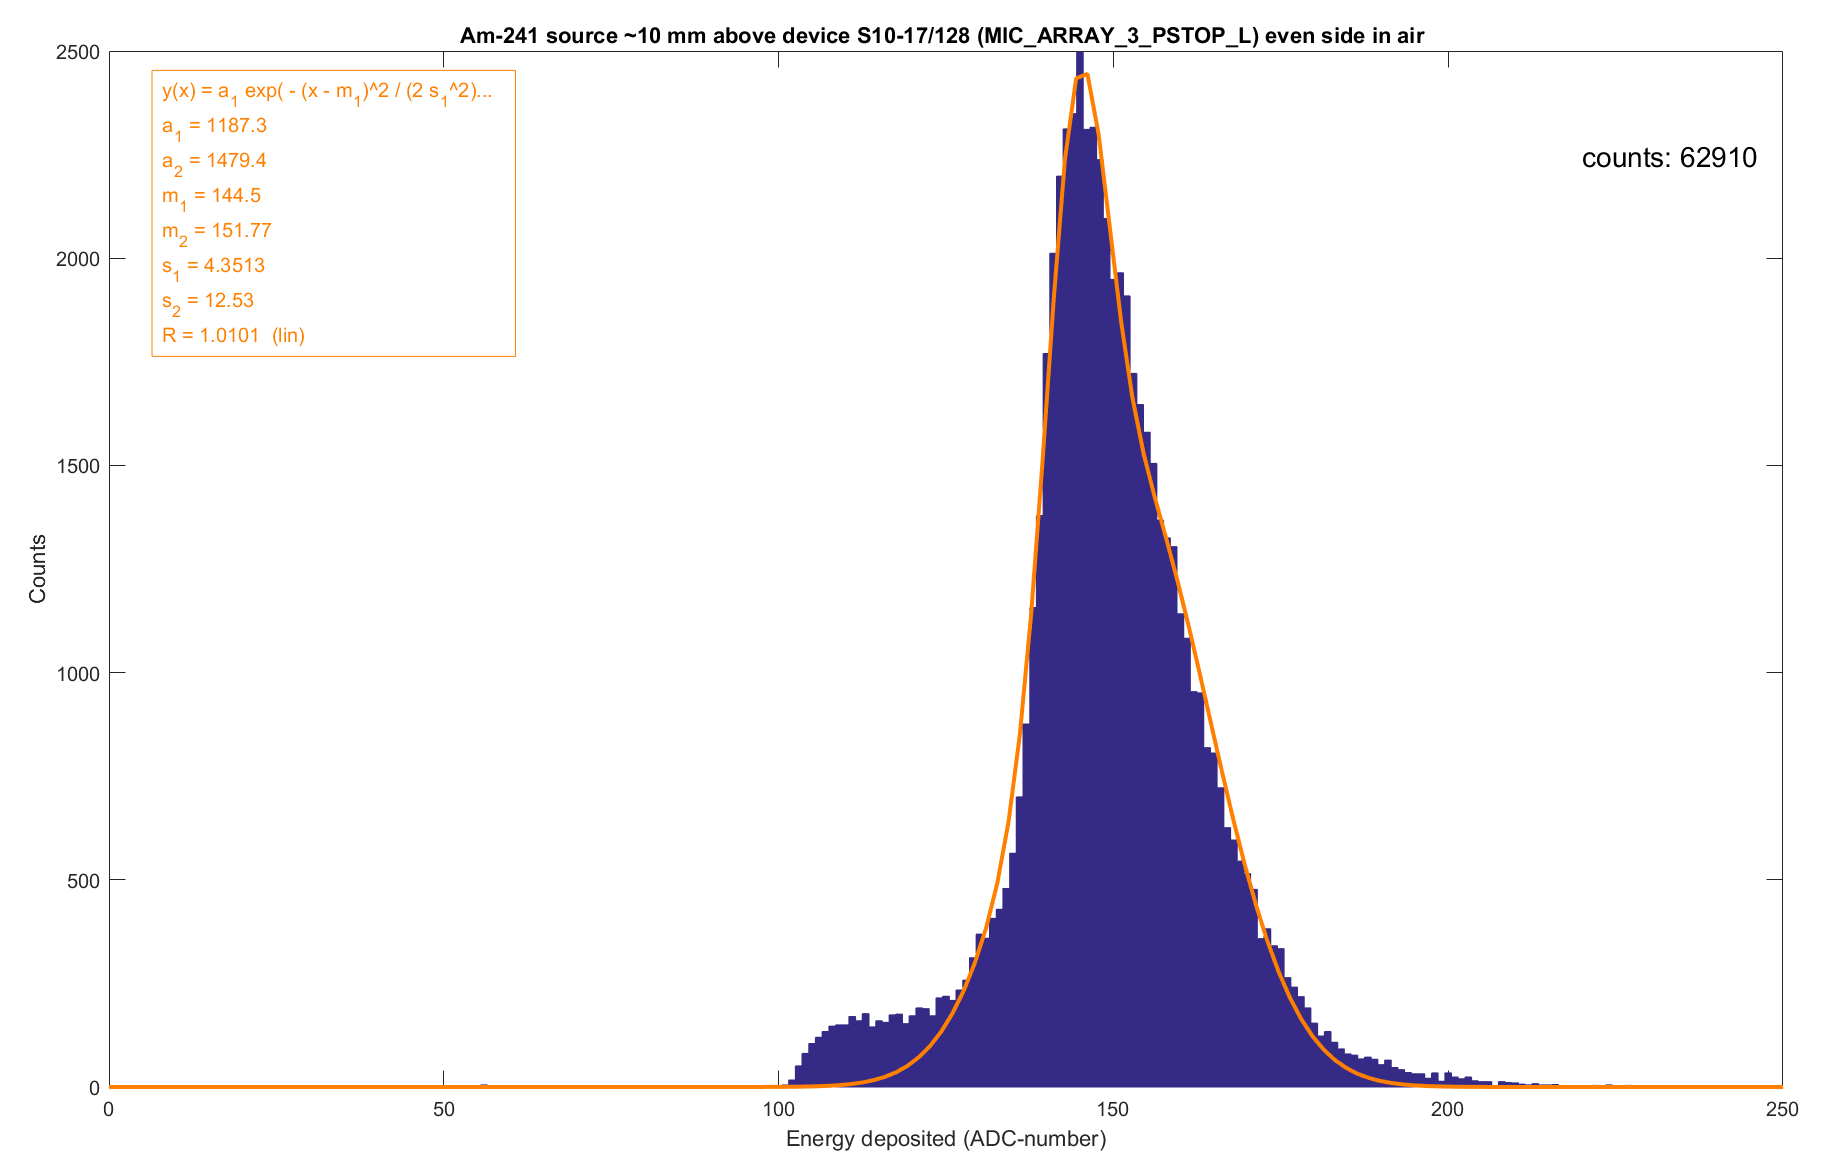
\includegraphics[width=\textwidth]{S10-17-128-even-10mm-1.png}
	\caption{Am-241 radiation measurement at 10 mm distance.}
	\label{fig-3dmimic-am-17-128-10}
\end{figure}

\begin{figure}[p]
	\centering
	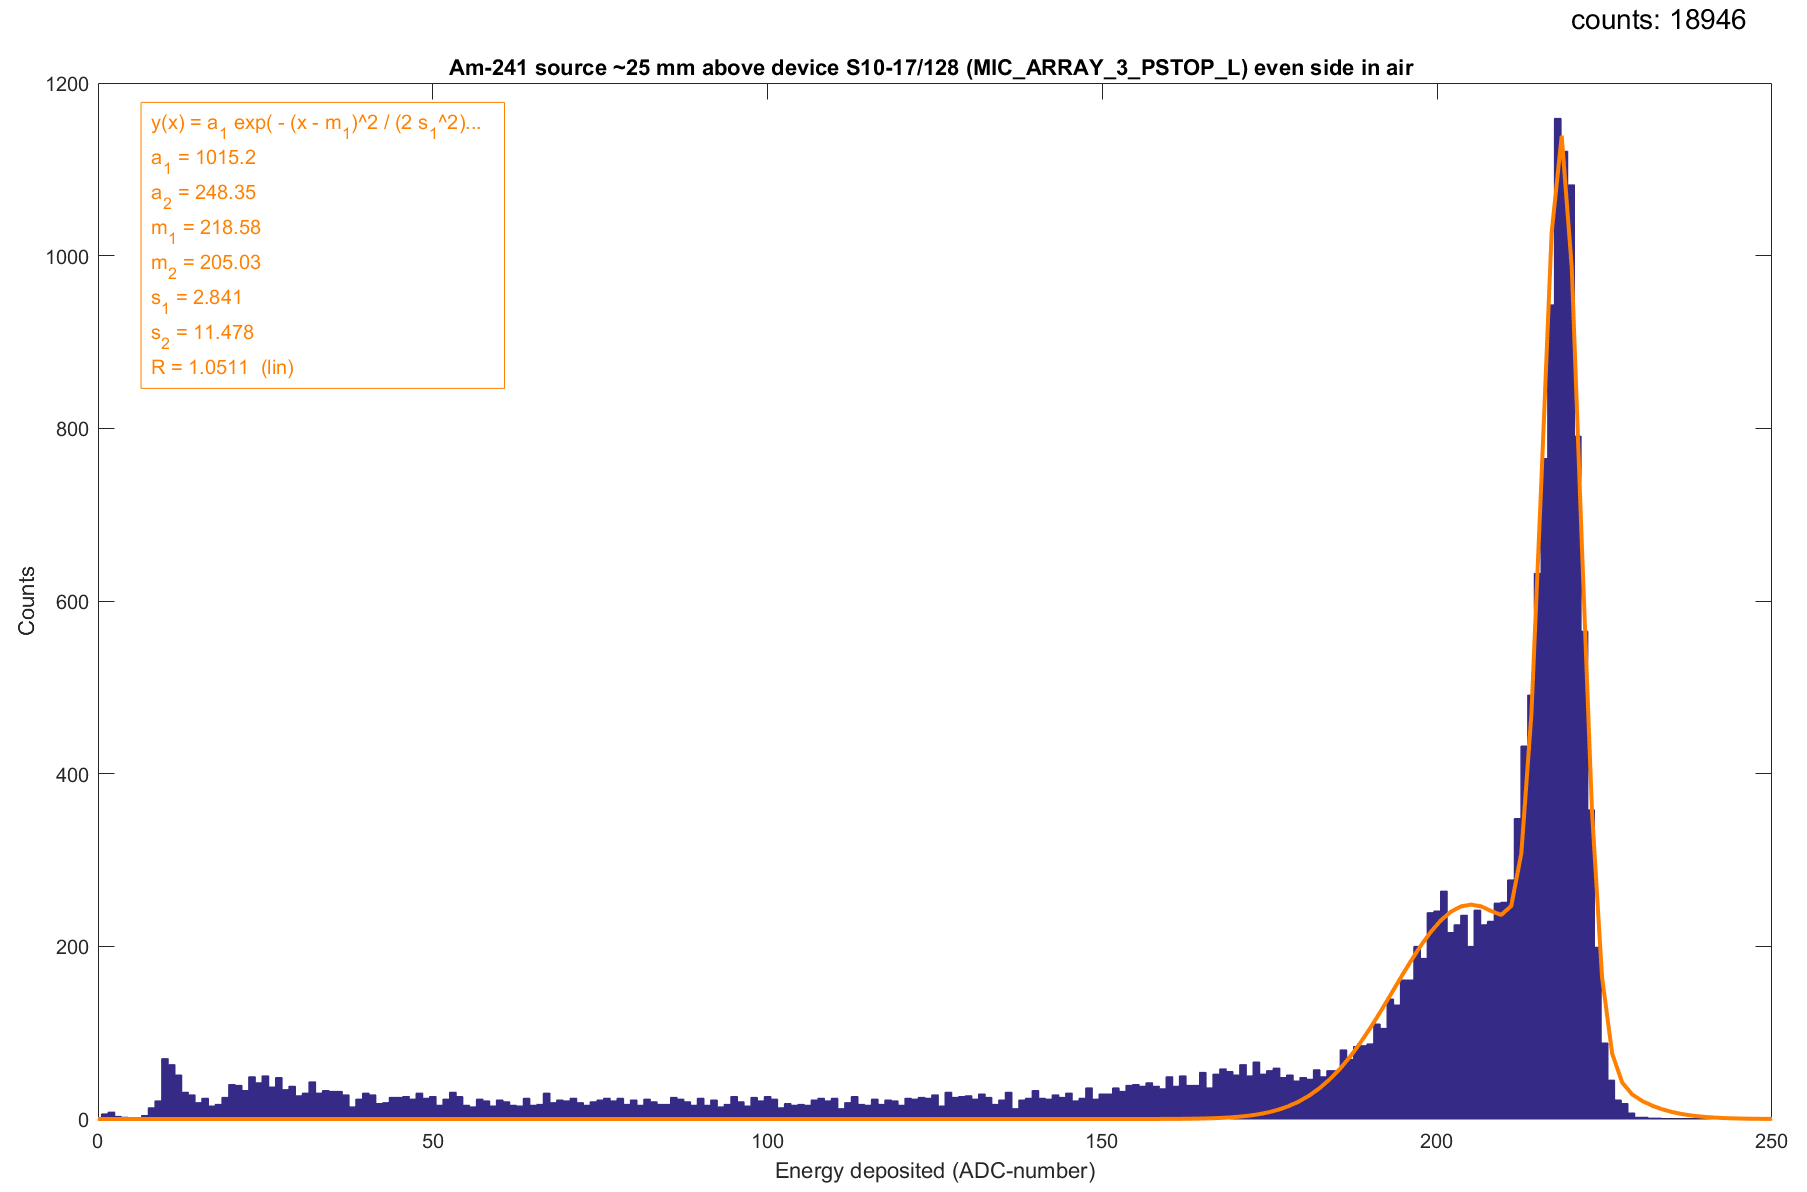
\includegraphics[width=\textwidth]{S10-17-128-even-25mm-1.png}
	\caption{Am-241 radiation measurement at 25 mm distance.}
	\label{fig-3dmimic-am-17-128-25}
\end{figure}


\end{document}